% Build twice here: pdflatex -interaction=nonstopmode -halt-on-error resume14An26w.tex
\documentclass[a4paper,10pt,pdflatex,ja=standard,jafont=ipaex-type1,
  magstyle=real,scale=1]{bxjsarticle}
\usepackage{lmodern}
\usepackage{amsmath,amssymb,mathtools}
\usepackage{geometry}
\geometry{reset,left=22mm,right=22mm,top=20mm,bottom=17mm,
  headheight=13pt,headsep=6mm,footskip=10mm}
\usepackage{xcolor}
\usepackage{enumitem}
\usepackage{array,booktabs,tabularx}
\usepackage{fancyhdr}
\usepackage{lastpage}
\usepackage{tikz}
\usetikzlibrary{arrows.meta,calc,decorations.pathreplacing}

\definecolor{ink}{HTML}{193A5C}
\definecolor{accent}{HTML}{237D82}
\definecolor{soft}{HTML}{EAF3F3}
\definecolor{muted}{HTML}{52616B}
\newcommand{\coursename}{解析学 II}
\newcommand{\handoutnumber}{14}
\pagestyle{fancy}
\fancyhf{}
\fancyhead[L]{\small\color{ink}\coursename{}・授業要約と演習}
\fancyhead[R]{\small\color{ink}第\handoutnumber 回}
\fancyfoot[C]{\small\color{ink}\thepage/\pageref{LastPage}}
\renewcommand{\headrulewidth}{0.3pt}
\setlength{\parindent}{0pt}
\setlength{\parskip}{2pt}
\setlength{\abovedisplayskip}{5pt}
\setlength{\belowdisplayskip}{5pt}
\setlength{\abovedisplayshortskip}{3pt}
\setlength{\belowdisplayshortskip}{4pt}
\setlist[itemize]{leftmargin=1.8em,itemsep=1pt,topsep=2pt,parsep=0pt}

\newcommand{\handouttitle}[1]{%
  \begin{center}
    {\Large\color{ink}#1}\par\vspace{3mm}
    {\color{accent}\rule{0.88\linewidth}{0.7pt}}
  \end{center}\vspace{-2mm}}
\newcommand{\handout}[2]{%
  \renewcommand{\handoutnumber}{#1}%
  \handouttitle{第#1回\quad #2}}
\newcommand{\topic}[1]{\par\vspace{5pt}%
  {\large\sffamily\mdseries\color{accent}#1}\par\vspace{2pt}}
\newcommand{\keybox}[1]{\par\vspace{3pt}\begingroup
  \setlength{\fboxsep}{4pt}%
  \colorbox{soft}{\parbox{\dimexpr\linewidth-2\fboxsep\relax}{\small #1}}%
  \endgroup\par\vspace{2pt}}
\newenvironment{problems}
  {\begin{enumerate}[leftmargin=2em,itemsep=3pt,topsep=3pt,parsep=0pt,
    font=\color{accent}]}
  {\end{enumerate}}


\newcommand{\examplelabel}[1]{{\sffamily\mdseries\color{ink}#1}}
\newcommand{\problemspace}{\par\vspace{5mm}}
\newcommand{\exercises}{%
  {\color{accent}\hrule height 0.7pt}\vspace{3pt}%
  \topic{演習問題（6題）}%
  {\small 領域と積分範囲を確認し、計算過程も書こう。図を描くと範囲を読み取りやすい。}\par}
\tikzset{
  handout diagram/.style={>={Stealth[length=3.2pt,width=3.2pt]},line join=round,
    every node/.style={font=\scriptsize,text=ink}},
  region/.style={fill=soft,draw=accent,semithick},
  slice/.style={accent,line width=1.8pt},
  guide/.style={muted,densely dashed,thin},
  axis/.style={->,ink,thin}}


% Review Q&A can also be used for actual student feedback when it is available.
\newcommand{\feedback}[2]{%
  \par\addvspace{8pt}\noindent\begin{minipage}{\linewidth}%
  {\color{ink}Q. #1}\par\vspace{2pt}%
  {\color{accent}A. }#2%
  \end{minipage}\par}

\begin{document}
\fontsize{10pt}{13.5pt}\selectfont
\setlength{\abovedisplayskip}{4pt}
\setlength{\belowdisplayskip}{4pt}
% Feedback section: add comments and responses here when available.
\fancyhead[L]{\small\color{ink}\coursename{}・フィードバック}
\handout{14}{前回のコメントへのフィードバック}
% \feedback{comment}{response}
\clearpage

% Previous small-test section: add the questions and solutions here.
\fancyhead[L]{\small\color{ink}\coursename{}・小テスト}
\fancyhead[R]{\small\color{ink}第13回}
\handouttitle{第13回\quad 小テスト}
% Questions and solutions are intentionally blank.
\clearpage

\fancyhead[L]{\small\color{ink}\coursename{}・授業要約と演習}
\fancyhead[R]{\small\color{ink}第\handoutnumber 回}
\handout{14}{ストークスとガウスの定理}\label{lesson-start}
\keybox{到達目標：循環にはストークス、閉曲面の流束にはガウスを選んで計算できる。
境界の向き・補助曲面・特異点を、図に書き込んでから式を立てよう。}

\topic{ストークスの定理：回転と境界の循環}
$S$ を境界を含むコンパクトな、向き付けられた区分的に滑らかな曲面とする。
$\vec F$ はその近傍で $C^1$ 級とする。
単位法線 $\vec n$ と境界 $\partial S$ の向きを右手の規則でそろえると
$$
 \oint_{\partial S}\vec F\cdot d\vec r
 =\iint_S(\nabla\times\vec F)\cdot\vec n\,dS.
$$
曲面内部の回転の総和が境界の循環に等しい。
同じ向きの境界をもつ別の曲面に置き換えると、計算が簡単になることがある。
平面 $z=0$、法線 $+z$ の場合はグリーンの定理になる。


\par\vspace{2pt}\noindent
\begin{minipage}[b]{0.48\linewidth}\centering
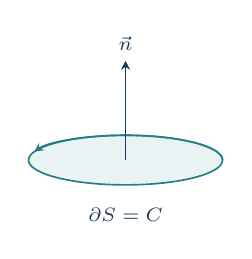
\begin{tikzpicture}[handout diagram,x=0.85cm,y=0.7cm]
\path[region] (0,0) ellipse (1.45 and 0.45);
 \draw[accent,->,semithick] (1.45,0) arc[start angle=0,end angle=160,x radius=1.45,y radius=0.45];
 \draw[->,ink,semithick] (0,0) -- (0,1.8) node[above] {$\vec n$};
 \node[below] at (0,-0.7) {$\partial S=C$};
\end{tikzpicture}\par
{\small\color{muted}境界 $C$ を張る円板}\par
\end{minipage}\hfill
\begin{minipage}[b]{0.48\linewidth}\centering
\begin{tikzpicture}[handout diagram,x=0.85cm,y=0.7cm]
\fill[soft] (-1.45,0) .. controls (-1.45,1.8) and (1.45,1.8) .. (1.45,0)
   arc[start angle=0,end angle=-180,x radius=1.45,y radius=0.45] -- cycle;
 \draw[accent] (-1.45,0) .. controls (-1.45,1.8) and (1.45,1.8) .. (1.45,0);
 \draw[accent] (1.45,0) arc[start angle=0,end angle=-180,x radius=1.45,y radius=0.45];
 \draw[guide] (1.45,0) arc[start angle=0,end angle=180,x radius=1.45,y radius=0.45];
 \draw[->,ink,semithick] (0,1.35) -- (0,2.1) node[above] {$\vec n$};
 \node[below] at (0,-0.7) {同じ境界 $C$};
\end{tikzpicture}\par
{\small\color{muted}場が両曲面の近傍で滑らかなら置き換えられる}\par
\end{minipage}
\par\vspace{2pt}

\topic{例：円板上の循環}
$\vec F=(-y,x,0)$、$S=\{z=h,\ x^2+y^2\le R^2\}$ を上向きに取ると
$$
 \nabla\times\vec F=(0,0,2),\qquad
 \oint_{\partial S}\vec F\cdot d\vec r
 =\iint_S2\,dS=2\pi R^2.
$$
一方 $\vec G=(yz,xz,xy)=\nabla(xyz)$ では、$\nabla\times\vec G=\vec0$。
したがって、$\mathbb R^3$ 内の任意の区分的に滑らかな閉曲線に沿う循環は0である。


\topic{ガウスの発散定理：発散と閉曲面の流束}
$V$ を区分的に滑らかな境界をもつ有界立体、$\vec F$ を $\overline V$ の近傍で
$C^1$ 級とする。境界の単位法線 $\vec n$ を外向きに取ると
$$
 \iint_{\partial V}\vec F\cdot\vec n\,dS
 =\iiint_V\nabla\cdot\vec F\,dV.
$$
立体内部の湧き出しの総量が、閉曲面を通って外へ出る流束に等しい。
開いた曲面へ使うときは、補助曲面を加えて閉じ、その流束を差し引く。


\par\vspace{2pt}\noindent
\begin{minipage}[b]{0.98\linewidth}\centering
\begin{tikzpicture}[handout diagram,x=0.8cm,y=0.65cm]
\path[region] (0,0) circle (1.3);
 \draw[guide] (0,0) ellipse (1.3 and 0.33);
 \foreach \t in {0,60,130,200,280}{
  \draw[->,ink,semithick] (\t:1.3) -- (\t:1.95);}
 \node at (0,0.55) {$V$};
 \node at (0,-0.55) {$\operatorname{div}\vec F$};
 \node[right] at (2.5,0.55) {外向きの閉曲面 $\partial V$};
 \node[right] at (2.5,-0.3) {内部の発散を積分する};
\end{tikzpicture}\par
{\small\color{muted}ガウスの定理では、境界が閉じていることと外向き法線を確認する}\par
\end{minipage}
\par\vspace{2pt}

\newpage
% Keep the remaining summary in the upper half of page 2.
\noindent\begin{minipage}[b][\dimexpr0.5\textheight-\parskip\relax][t]{\linewidth}
\topic{例：球面の流束と対称性}
$\vec F=(x,y,z)$ なら $\nabla\cdot\vec F=3$。半径 $R>0$ の球 $V$ について
$$
 \iint_{\partial V}\vec F\cdot\vec n\,dS
 =3\operatorname{Vol}(V)=4\pi R^3.
$$
$\vec H=(x^2,y^2,z^2)$ なら $\nabla\cdot\vec H=2x+2y+2z$。
原点中心の球では対称性から各項の体積積分が0となり、全流束も0である。


\topic{定理を使い分ける}
循環の計算には回転とストークス、閉曲面の流束には発散とガウスを用いる。
$$
 \text{境界曲線の循環}\ \longleftrightarrow\ \text{曲面上の回転},\qquad
 \text{閉曲面の流束}\ \longleftrightarrow\ \text{立体内の発散}.
$$
場に特異点があれば、定理の仮定を満たす領域へ分ける。
境界の向き・法線の向き・補助曲面の寄与を式に書いてから計算する。
\keybox{境界積分と内部積分を結ぶ公式には、滑らかさと向きの条件がある。特異点を含む立体に発散定理を直接使わない。}

\par\vspace{2pt}\noindent
\begin{minipage}[b]{0.48\linewidth}\centering
\begin{tikzpicture}[handout diagram,x=0.85cm,y=0.6cm]
\fill[soft] (-1.3,0) .. controls (-1.3,1.6) and (1.3,1.6) .. (1.3,0)
   arc[start angle=0,end angle=-180,x radius=1.3,y radius=0.36] -- cycle;
 \draw[accent] (-1.3,0) .. controls (-1.3,1.6) and (1.3,1.6) .. (1.3,0);
 \filldraw[fill=accent!18,draw=accent] (0,0) ellipse (1.3 and 0.36);
 \draw[->,ink] (0,1.2) -- (0,1.95) node[above] {外向き};
 \draw[->,ink] (0,0) -- (0,-0.95) node[below] {底面は下向き};
\end{tikzpicture}\par
{\small\color{muted}開いた曲面は、底面を加えて閉じる}\par
\end{minipage}\hfill
\begin{minipage}[b]{0.48\linewidth}\centering
\begin{tikzpicture}[handout diagram,x=0.85cm,y=0.6cm]
\path[region,even odd rule] (0,0) circle (1.35) (0,0) circle (0.5);
 \fill[ink] (0,0) circle (1.5pt);
 \draw[->,ink] (1.35,0) -- (2,0);
 \draw[->,ink] (0,0.5) -- (0,0.12);
 \node[above left] at (-0.15,0) {特異点};
 \node[right] at (0.65,0.75) {内側も境界};
 \node[below] at (0,-1.7) {球殻の断面};
\end{tikzpicture}\par
{\small\color{muted}小球を除くと、その内側の法線は原点へ向く}\par
\end{minipage}
\par\vspace{2pt}

\end{minipage}\par\nointerlineskip
% Keep the exercises and writing space in the lower half of page 2.
\noindent\begin{minipage}[b][0.5\textheight][t]{\linewidth}
\exercises
\begin{problems}
\item $\vec F=(-y,x,0)$、$C=\{z=2,\ x^2+y^2=1\}$ を $+z$ 側から見て反時計回りに取る。$\oint_C\vec F\cdot d\vec r$ をストークスの定理で求めよ。
\problemspace

\item $S=\{z=1-x^2-y^2,\ x^2+y^2\le1\}$ を上向きに取り、$\vec F=(-y/2,x/2,0)$ とする。$\partial S$ の向きを指定し、境界の循環と回転の面積分が一致することを確かめよ。
\problemspace

\item 半径 $R>0$ の球面を外向きに取る。$\vec F=(x,y,z)$ の流束を、ガウスの定理と直接の球面上の計算で求めよ。
\problemspace

\item $V=[0,1]^3$、$\vec F=(xy,yz,zx)$ とする。外向きの全流束を発散定理で求め、6面の寄与を足す方法でも確かめよ。
\problemspace

\item 単位上半球の曲面を外向きに取り、$\vec F=(0,0,z)$ とする。底面を加えて閉曲面を作り、上半球の曲面を通る流束を求めよ。
\problemspace

\item $\vec F=\vec r/|\vec r|^3$（$\vec r=(x,y,z)\ne\vec0$）の発散を求めよ。原点中心の半径 $R$ の球面を通る流束を直接計算し、球全体に発散定理を適用できない理由を説明せよ。
\problemspace
\end{problems}
\end{minipage}

\newpage
\handouttitle{第14回\quad 演習問題の解答}
{\small 設定した範囲と条件も確認しながら、計算を振り返ろう。}\par
\begin{problems}
\setlength{\itemsep}{7pt}
\item $z=2$ の単位円板を上向きに取れば、指定された反時計回りと整合する。
$\nabla\times\vec F=(0,0,2)$ なので、ストークスの定理から
$$
 \oint_C\vec F\cdot d\vec r=\iint_S2\,dS=2\pi.
$$

\item 上向き法線に対応する境界は、$+z$ 側から見て反時計回り。
$\partial S$ は $z=0$ の単位円周なので、$\vec r(t)=(\cos t,\sin t,0)$ として
$$
 \oint_{\partial S}\vec F\cdot d\vec r=\int_0^{2\pi}\frac12\,dt=\pi.
$$
一方、$\nabla\times\vec F=(0,0,1)$、上向き面積ベクトルは $(2x,2y,1)\,dx\,dy$。
回転の面積分も $\iint_{x^2+y^2\le1}1\,dx\,dy=\pi$ となり一致する。

\item 発散は3なので、ガウスの定理では
$$
 \iint_{\partial V}\vec F\cdot\vec n\,dS
 =3\cdot\frac{4\pi R^3}{3}=4\pi R^3.
$$
直接の計算では $\vec n=(x,y,z)/R$、$\vec F\cdot\vec n=R$。
したがって流束は $R\cdot\operatorname{Area}(\partial V)=R\cdot4\pi R^2=4\pi R^3$。

\item $\nabla\cdot\vec F=y+z+x$ より、全流束は
$$
 \iiint_{[0,1]^3}(x+y+z)\,dV=\frac12+\frac12+\frac12=\frac32.
$$
直接には、$x=1$、$y=1$、$z=1$ の各面の寄与が順に
$\int_0^1\int_0^1y\,dy\,dz=1/2$、$\int_0^1\int_0^1z\,dz\,dx=1/2$、
$\int_0^1\int_0^1x\,dx\,dy=1/2$。
$x=0,y=0,z=0$ の3面では対応成分が0。和は $3/2$ と一致する。

\item 上半球と底面で囲む立体を $V$ とすると、$\nabla\cdot\vec F=1$ より全流束は
$\operatorname{Vol}(V)=2\pi/3$。底面では $z=0$ のため $\vec F=\vec0$ で、流束も0。
したがって、上半球の曲面を通る外向き流束は $2\pi/3$ である。

\item $s=|\vec r|>0$ とおけば、各成分を微分して
$$
 \nabla\cdot\left(\frac{\vec r}{s^3}\right)
 =\frac3{s^3}-\frac{3(x^2+y^2+z^2)}{s^5}=0.
$$
半径 $R$ の球面では $\vec F\cdot\vec n=1/R^2$ なので流束は $4\pi$。
原点で場が定義されないため、球全体では発散定理の仮定を満たさない。
原点の小球を除いた球殻なら、内側の流束 $-4\pi$ も加わり、全流束は0になる。
\end{problems}
\keybox{ストークスでは法線と境界の向きを対応させる。ガウスでは全境界を外向きにそろえ、補助面や内側の境界の寄与も含めよう。}
\end{document}
